% Docker MCP Gateway: Enabling MCP-as-a-Service for Enterprise AI Integration
% Technical Paper - December 2025
\documentclass[11pt,letterpaper]{article}

% Packages
\usepackage[utf8]{inputenc}
\usepackage[margin=1in]{geometry}
\usepackage{amsmath,amssymb}
\usepackage{algorithm}
\usepackage{algorithmic}
\usepackage{listings}
\usepackage{xcolor}
\usepackage{hyperref}
\usepackage{booktabs}
\usepackage{graphicx}
\usepackage{tikz}
\usepackage{fancyhdr}
\usepackage{enumitem}

\usetikzlibrary{shapes.geometric, arrows, positioning, fit, backgrounds}

% Hyperref setup
\hypersetup{
    colorlinks=true,
    linkcolor=blue,
    citecolor=blue,
    urlcolor=blue,
    pdftitle={Docker MCP Gateway: Enabling MCP-as-a-Service},
    pdfauthor={NOAA EMC Global Workflow MCP Team},
    pdfkeywords={MCP, Docker, Gateway, AI Integration, Model Context Protocol}
}

% Code listing setup
\lstset{
    basicstyle=\ttfamily\footnotesize,
    breaklines=true,
    frame=single,
    captionpos=b,
    numbers=left,
    numberstyle=\tiny\color{gray},
    keywordstyle=\color{blue},
    commentstyle=\color{green!60!black},
    stringstyle=\color{red},
    backgroundcolor=\color{gray!5}
}

% Header/Footer
\pagestyle{fancy}
\fancyhf{}
\rhead{Docker MCP Gateway}
\lhead{NOAA EMC Global Workflow Team}
\cfoot{\thepage}

% Title information
\title{\textbf{Docker MCP Gateway:} \\
       \textbf{Enabling MCP-as-a-Service for Enterprise AI Integration} \\[0.5em]
       \large A Technical Guide to Multi-Client Model Context Protocol Deployment}

\author{
    NOAA EMC Global Workflow MCP Team \\
    Environmental Modeling Center \\
    National Oceanic and Atmospheric Administration \\
    \texttt{Terry.McGuinness@noaa.gov}
}

\date{December 15, 2025}

\begin{document}

\maketitle

\begin{abstract}
The Model Context Protocol (MCP) has emerged as a critical standard for enabling AI assistants to interact with external tools and data sources. However, the default stdio-based transport mechanism limits MCP servers to single-client, single-session usage patterns. This paper presents the \textbf{Docker MCP Gateway}---an open-source solution that transforms containerized MCP servers into multi-client services accessible via HTTP/SSE transports. We describe the architectural challenges of MCP-as-a-Service deployment, analyze the gateway's security model, and demonstrate practical implementation within the NOAA Global Workflow AI assistance infrastructure. Our deployment enables simultaneous access from VS Code Copilot, Claude Desktop, LangFlow, and custom applications to a unified 32-tool MCP server backed by vector and graph databases. This work addresses the critical gap between MCP's powerful tool integration capabilities and enterprise requirements for scalable, multi-tenant AI service deployment.

\textbf{Keywords:} Model Context Protocol, Docker, Gateway Pattern, AI Infrastructure, Multi-Client Services, Container Orchestration, RAG Systems
\end{abstract}

%===============================================================================
\section{Introduction}
%===============================================================================

\subsection{The MCP Revolution}

The Model Context Protocol (MCP), introduced by Anthropic in late 2024, represents a paradigm shift in how AI assistants interact with external systems. Unlike traditional approaches where each AI application implements custom integrations, MCP provides a standardized protocol enabling:

\begin{itemize}[noitemsep]
    \item \textbf{Tool Discovery}: AI clients can enumerate available tools dynamically
    \item \textbf{Structured Invocation}: Type-safe parameter passing with JSON Schema validation
    \item \textbf{Resource Access}: Standardized file, database, and API access patterns
    \item \textbf{Prompt Templates}: Reusable prompt components shared across applications
\end{itemize}

The MCP specification defines a JSON-RPC 2.0 based protocol that enables AI clients (Claude, VS Code Copilot, etc.) to communicate with \textit{MCP servers}---specialized processes that expose tools, resources, and prompts to the AI.

\subsection{The Single-Client Limitation}

Despite MCP's power, its default transport mechanism---standard input/output (stdio)---creates a fundamental limitation: \textbf{one client, one session, one server instance}. This design, while elegant for local development, prevents:

\begin{enumerate}[noitemsep]
    \item Multiple developers sharing a common MCP server
    \item Integration with web-based tools (LangFlow, n8n, custom dashboards)
    \item Centralized logging and monitoring of tool invocations
    \item Load balancing across multiple server instances
    \item Separation of MCP server deployment from client workstations
\end{enumerate}

For enterprise deployments requiring centralized AI tool infrastructure, this limitation is critical.

\subsection{Our Contribution}

This paper presents:

\begin{enumerate}[noitemsep]
    \item Analysis of the \textbf{Docker MCP Gateway} architecture and its role in enabling MCP-as-a-Service
    \item Practical deployment patterns for \textbf{containerized MCP servers} with database dependencies
    \item Security considerations for \textbf{multi-client MCP access}
    \item Implementation details from our \textbf{NOAA Global Workflow} deployment with 32 tools serving multiple AI clients simultaneously
\end{enumerate}

%===============================================================================
\section{Background: MCP Transport Mechanisms}
%===============================================================================

\subsection{Standard I/O Transport (Default)}

The MCP specification's primary transport uses Unix standard streams:

\begin{lstlisting}[language=bash,caption={Stdio MCP Communication}]
# Client spawns server process
node mcp-server.js

# JSON-RPC messages flow through stdin/stdout
< {"jsonrpc":"2.0","id":1,"method":"initialize",...}
> {"jsonrpc":"2.0","id":1,"result":{...}}
\end{lstlisting}

\textbf{Advantages}:
\begin{itemize}[noitemsep]
    \item Simple process management
    \item No network configuration required
    \item Inherent security (local process only)
\end{itemize}

\textbf{Limitations}:
\begin{itemize}[noitemsep]
    \item Single client per server instance
    \item Client must manage server lifecycle
    \item No remote access capability
\end{itemize}

\subsection{Server-Sent Events (SSE) Transport}

MCP also supports SSE for network-based communication:

\begin{lstlisting}[language=bash,caption={SSE MCP Communication}]
# Server listens on HTTP port
POST /mcp HTTP/1.1
Content-Type: application/json

{"jsonrpc":"2.0","id":1,"method":"tools/list"}

# Server responds with SSE stream
event: message
data: {"jsonrpc":"2.0","id":1,"result":{"tools":[...]}}
\end{lstlisting}

\textbf{Advantages}:
\begin{itemize}[noitemsep]
    \item Network-accessible
    \item Multiple clients possible (with session management)
    \item Standard HTTP infrastructure compatibility
\end{itemize}

\textbf{Limitations}:
\begin{itemize}[noitemsep]
    \item Server must implement HTTP handling
    \item Session state management complexity
    \item Security considerations (authentication, CORS)
\end{itemize}

\subsection{The Gateway Pattern}

The \textbf{Docker MCP Gateway} bridges these transports: it accepts HTTP/SSE connections from multiple clients and translates them to stdio connections with containerized MCP servers. This enables MCP-as-a-Service without modifying existing stdio-based servers.

%===============================================================================
\section{Docker MCP Gateway Architecture}
%===============================================================================

\subsection{System Overview}

\begin{figure}[ht]
\centering
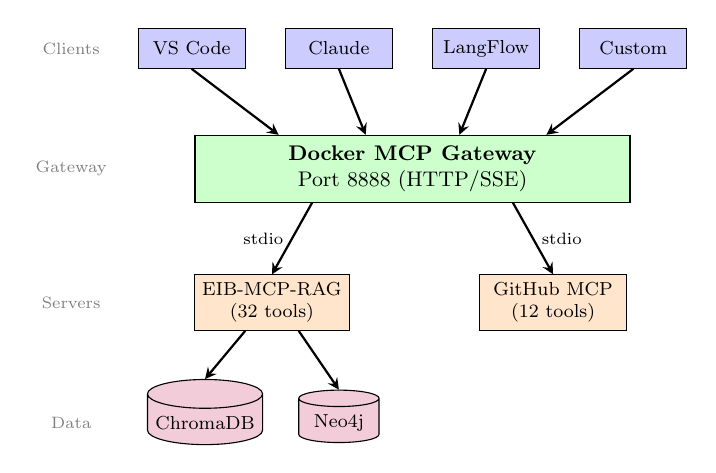
\begin{tikzpicture}[
    scale=0.85,
    every node/.style={transform shape},
    client/.style={rectangle, draw, fill=blue!20, minimum width=1.6cm, minimum height=0.6cm, font=\footnotesize},
    gateway/.style={rectangle, draw, fill=green!20, minimum width=6.5cm, minimum height=1cm, font=\small, align=center},
    server/.style={rectangle, draw, fill=orange!20, minimum width=2.2cm, minimum height=0.8cm, font=\footnotesize, align=center},
    db/.style={cylinder, draw, fill=purple!20, minimum width=1.2cm, minimum height=0.7cm, font=\footnotesize, shape border rotate=90, aspect=0.25},
    arrow/.style={->, thick, >=stealth}
]

% Row 1: Clients
\node[client] at (0,5) (vscode) {VS Code};
\node[client] at (2.2,5) (claude) {Claude};
\node[client] at (4.4,5) (langflow) {LangFlow};
\node[client] at (6.6,5) (custom) {Custom};

% Row 2: Gateway (centered under clients, wider)
\node[gateway] at (3.3,3.2) (gateway) {\textbf{Docker MCP Gateway}\\Port 8888 (HTTP/SSE)};

% Row 3: MCP Servers
\node[server] at (1.2,1.2) (eib) {EIB-MCP-RAG\\(32 tools)};
\node[server] at (5.4,1.2) (github) {GitHub MCP\\(12 tools)};

% Row 4: Databases (under EIB server only)
\node[db] at (0.2,-0.6) (chromadb) {ChromaDB};
\node[db] at (2.2,-0.6) (neo4j) {Neo4j};

% Client arrows to gateway - angled like lower levels
\draw[arrow] (vscode.south) -- ([xshift=-2cm]gateway.north);
\draw[arrow] (claude.south) -- ([xshift=-0.7cm]gateway.north);
\draw[arrow] (langflow.south) -- ([xshift=0.7cm]gateway.north);
\draw[arrow] (custom.south) -- ([xshift=2cm]gateway.north);

% Gateway to servers - angled
\draw[arrow] ([xshift=-1.5cm]gateway.south) -- node[left, font=\scriptsize] {stdio} (eib.north);
\draw[arrow] ([xshift=1.5cm]gateway.south) -- node[right, font=\scriptsize] {stdio} (github.north);

% EIB to databases - angled
\draw[arrow] ([xshift=-0.4cm]eib.south) -- (chromadb.north);
\draw[arrow] ([xshift=0.4cm]eib.south) -- (neo4j.north);

% Labels for layers
\node[font=\scriptsize, gray] at (-1.8,5) {Clients};
\node[font=\scriptsize, gray] at (-1.8,3.2) {Gateway};
\node[font=\scriptsize, gray] at (-1.8,1.2) {Servers};
\node[font=\scriptsize, gray] at (-1.8,-0.6) {Data};

\end{tikzpicture}
\caption{Docker MCP Gateway Architecture: Multiple AI clients connect via HTTP/SSE to the gateway, which translates requests to stdio-based MCP servers running in Docker containers.}
\label{fig:architecture}
\end{figure}

The gateway operates as a protocol bridge:

\begin{enumerate}[noitemsep]
    \item \textbf{Client Layer}: Multiple AI clients connect via HTTP/SSE
    \item \textbf{Gateway Layer}: Manages sessions, authentication, and routing
    \item \textbf{Server Layer}: Containerized MCP servers accessed via Docker stdio
    \item \textbf{Data Layer}: Backend databases (vector, graph, relational)
\end{enumerate}

\subsection{Key Components}

\subsubsection{Container Discovery}

The gateway discovers MCP servers through Docker image labels:

\begin{lstlisting}[caption={MCP Server Discovery Label}]
LABEL io.docker.server.metadata='{
  "name": "eib-mcp-rag",
  "title": "EIB MCP RAG Server",
  "description": "AI-powered MCP server with RAG",
  "type": "image",
  "image": "eib-mcp-rag:latest"
}'
\end{lstlisting}

This label enables automatic server registration when images are pulled or built.

\subsubsection{Session Management}

Each client connection receives a unique session:

\begin{lstlisting}[language=bash,caption={Session Initialization}]
POST /mcp HTTP/1.1
Authorization: Bearer <token>
Content-Type: application/json

{"jsonrpc":"2.0","id":1,"method":"initialize",...}

# Response includes session ID
event: message
id: YMXXJUBCRW5VJHR5XJY74MR3VP_0
data: {"jsonrpc":"2.0","id":1,"result":{...}}
\end{lstlisting}

Sessions maintain state for multi-turn tool interactions.

\subsubsection{Container Lifecycle}

The gateway manages container lifecycle automatically:

\begin{itemize}[noitemsep]
    \item \textbf{Startup}: Container spawned on first tool invocation
    \item \textbf{Communication}: JSON-RPC via Docker's stdio attachment
    \item \textbf{Cleanup}: Container removed after session ends (unless \texttt{--long-lived})
\end{itemize}

%===============================================================================
\section{Security Model}
%===============================================================================

\subsection{Network Isolation}

A critical security feature: the gateway runs MCP server containers in \textbf{network isolation} by default. Containers cannot access:

\begin{itemize}[noitemsep]
    \item Host network interfaces
    \item Other containers
    \item External services
\end{itemize}

This prevents malicious tools from exfiltrating data or attacking internal services.

\subsection{Authentication}

The gateway supports bearer token authentication:

\begin{lstlisting}[language=bash,caption={Gateway Authentication}]
# Set token via environment
export MCP_GATEWAY_AUTH_TOKEN="secret-token-value"

# Start gateway
docker mcp gateway run --port 8888 --transport streamable-http

# Clients must include token
curl -H "Authorization: Bearer secret-token-value" \
     -X POST http://localhost:8888/mcp
\end{lstlisting}

\subsection{Resource Limits}

Per-container resource constraints prevent denial-of-service:

\begin{lstlisting}[language=bash,caption={Resource Constraints}]
docker mcp gateway run \
  --cpus 1 \
  --memory 2Gb \
  --servers docker://eib-mcp-rag:latest
\end{lstlisting}

\subsection{Challenge: Database Connectivity}

Network isolation creates a challenge for MCP servers requiring database access. Our RAG-enabled server needs ChromaDB and Neo4j connections. Solutions:

\begin{enumerate}[noitemsep]
    \item \textbf{Gateway Bypass}: Run container directly on shared network (our approach)
    \item \textbf{Remote Endpoints}: Configure databases with public endpoints
    \item \textbf{Sidecar Pattern}: Deploy databases alongside MCP container
\end{enumerate}

%===============================================================================
\section{Implementation: NOAA Global Workflow Deployment}
%===============================================================================

\subsection{System Context}

Our deployment supports AI-assisted development of the NOAA Global Forecast System (GFS)---operational weather prediction infrastructure processing petabytes of atmospheric data daily. The MCP server provides:

\begin{itemize}[noitemsep]
    \item \textbf{32 Tools}: Code analysis, documentation search, compliance checking
    \item \textbf{14,854 Documents}: Indexed in ChromaDB vector database
    \item \textbf{85,894 Relationships}: Code dependency graph in Neo4j
    \item \textbf{Multiple Clients}: VS Code Copilot, Claude Desktop, LangFlow
\end{itemize}

\subsection{Container Configuration}

Our Dockerfile includes gateway metadata:

\begin{lstlisting}[language=bash,caption={Dockerfile with Gateway Support}]
FROM node:20-slim

# ... build steps ...

# Gateway discovery label (JSON format)
LABEL io.docker.server.metadata='{ \
  "name":"eib-mcp-rag", \
  "title":"EIB MCP RAG Server", \
  "description":"AI-powered MCP server with RAG", \
  "type":"image", \
  "image":"eib-mcp-rag:latest" \
}'

CMD ["node", "src/UnifiedMCPServer.js", "full"]
\end{lstlisting}

\subsection{Network Architecture}

Due to database requirements, we deploy with explicit network configuration:

\begin{lstlisting}[language=bash,caption={Production Container Deployment}]
# Create shared network
docker network create mcp-network

# Start databases
docker run -d --network mcp-network \
  --name chromadb chromadb/chroma:latest

docker run -d --network mcp-network \
  --name neo4j neo4j:5-community

# Start MCP server on same network
docker run -d --network mcp-network \
  --name eib-mcp-rag \
  -e CHROMADB_HOST=chromadb \
  -e CHROMADB_PORT=8000 \
  -e NEO4J_URI=bolt://neo4j:7687 \
  eib-mcp-rag:latest
\end{lstlisting}

\subsection{Gateway Deployment}

For multi-client access, we run the gateway in streaming mode:

\begin{lstlisting}[language=bash,caption={Gateway Startup}]
export MCP_GATEWAY_AUTH_TOKEN="$(openssl rand -hex 32)"

docker mcp gateway run \
  --servers docker://eib-mcp-rag:latest \
  --port 8888 \
  --transport streamable-http \
  --verbose
\end{lstlisting}

Gateway output confirms tool discovery:

\begin{lstlisting}[language=bash,caption={Gateway Initialization Output}]
- Those servers are enabled: eib-mcp-rag
- Listing MCP tools...
  > eib-mcp-rag: (32 tools)
> 32 tools listed in 2.65s
> Start streaming server on port 8888
> Gateway URL: http://localhost:8888/mcp
\end{lstlisting}

\subsection{Client Configuration}

\subsubsection{VS Code MCP Extension}

\begin{lstlisting}[caption={VS Code mcp.json Configuration}]
{
  "servers": {
    "eib-mcp-rag-gateway": {
      "type": "sse",
      "url": "http://localhost:8888/mcp",
      "headers": {
        "Authorization": "Bearer ${MCP_GATEWAY_AUTH_TOKEN}"
      }
    }
  }
}
\end{lstlisting}

\subsubsection{LangFlow Integration}

LangFlow connects via its MCP component, enabling visual workflow construction with MCP tools as nodes.

%===============================================================================
\section{Operational Considerations}
%===============================================================================

\subsection{Tool Verification}

We verify tool availability through the gateway:

\begin{lstlisting}[language=bash,caption={Tool List Verification}]
curl -X POST http://localhost:8888/mcp \
  -H "Authorization: Bearer $TOKEN" \
  -H "Content-Type: application/json" \
  -d '{"jsonrpc":"2.0","id":1,"method":"tools/list"}'

# Response includes all 32 tools
\end{lstlisting}

\subsection{Health Monitoring}

Our MCP server includes health check tools:

\begin{lstlisting}[caption={Health Check Tool Call}]
{
  "jsonrpc": "2.0",
  "id": 2,
  "method": "tools/call",
  "params": {
    "name": "get_knowledge_base_status",
    "arguments": {"include_graph": true}
  }
}
\end{lstlisting}

Response confirms database connectivity:

\begin{lstlisting}[caption={Health Check Response}]
Vector Database (ChromaDB):
  - Collections: 12
  - Total Documents: 14,854
  - Status: Healthy

Graph Database (Neo4j):
  - Total Relationships: 85,894
  - Status: Healthy
\end{lstlisting}

\subsection{Provisioning Automation}

We automated gateway deployment in our provisioning system:

\begin{lstlisting}[language=bash,caption={Provisioning Script (excerpt)}]
# 11-docker-mcp-gateway.sh

# Install Go compiler
curl -sLO "https://go.dev/dl/go1.23.4.linux-amd64.tar.gz"
tar -C /usr/local -xzf go1.23.4.linux-amd64.tar.gz

# Build docker-mcp plugin
git clone https://github.com/docker/mcp-gateway.git
cd mcp-gateway
go build -o docker-mcp ./cmd/docker-mcp

# Install plugin
cp docker-mcp ~/.docker/cli-plugins/

# Build MCP server image
docker compose -f docker-compose.mcp-standalone.yaml build
\end{lstlisting}

%===============================================================================
\section{Lessons Learned}
%===============================================================================

\subsection{Docker CE vs Docker Desktop}

A critical finding: the \texttt{docker-mcp} plugin initially only worked with Docker Desktop due to API differences. Pull Request \#301 (merged December 12, 2025) added Docker CE support. \textbf{Building from source after this merge is required for Docker CE deployments.}

\subsection{Label Format}

The \texttt{io.docker.server.metadata} label must use \textbf{JSON format}, not YAML. Multi-line YAML with escaped newlines causes parsing failures:

\begin{lstlisting}[language=bash,caption={Label Format Comparison}]
# WRONG - causes parsing errors
LABEL io.docker.server.metadata="name: eib\ntitle: EIB"

# CORRECT - JSON format
LABEL io.docker.server.metadata='{"name":"eib","title":"EIB"}'
\end{lstlisting}

\subsection{Network Isolation Trade-offs}

Gateway security isolation prevents database access. For stateful MCP servers requiring backend services, direct network deployment (bypassing gateway container management) provides the necessary connectivity while maintaining protocol translation benefits.

%===============================================================================
\section{Future Work}
%===============================================================================

\begin{enumerate}[noitemsep]
    \item \textbf{Gateway Network Configuration}: Propose upstream feature for gateway to attach containers to specified networks
    \item \textbf{Multi-Tenant Authentication}: Integrate with institutional identity providers (OAuth, SAML)
    \item \textbf{Tool-Level Authorization}: Fine-grained access control per tool per user
    \item \textbf{Observability}: Distributed tracing for tool invocations across sessions
    \item \textbf{High Availability}: Gateway clustering with session affinity
\end{enumerate}

%===============================================================================
\section{Conclusion}
%===============================================================================

The Docker MCP Gateway transforms the Model Context Protocol from a single-client development tool into enterprise-ready infrastructure. By bridging stdio and HTTP/SSE transports, it enables:

\begin{itemize}[noitemsep]
    \item \textbf{Multi-Client Access}: Multiple AI assistants sharing common tools
    \item \textbf{Centralized Deployment}: MCP servers as managed services
    \item \textbf{Security Controls}: Authentication, resource limits, network isolation
    \item \textbf{Container Benefits}: Reproducible builds, version management, scaling
\end{itemize}

Our NOAA Global Workflow deployment demonstrates production viability: 32 tools serving multiple clients with sub-3-second initialization. The combination of vector database (14,854 documents) and graph database (85,894 relationships) provides AI assistants with comprehensive codebase understanding through a unified MCP interface.

As MCP adoption accelerates, gateway patterns will become essential infrastructure for organizations seeking to operationalize AI-assisted development at scale. The open-source Docker MCP Gateway provides a foundation for this transformation.

%===============================================================================
\section*{Acknowledgments}
%===============================================================================

This work was conducted at NOAA's Environmental Modeling Center as part of the Global Workflow modernization initiative. We thank the Docker team for open-sourcing the MCP Gateway and the Anthropic team for the Model Context Protocol specification.

%===============================================================================
\section*{References}
%===============================================================================

\begin{enumerate}[noitemsep]
    \item Anthropic. ``Model Context Protocol Specification.'' \url{https://spec.modelcontextprotocol.io/}, 2024.
    \item Docker, Inc. ``Docker MCP Gateway.'' \url{https://github.com/docker/mcp-gateway}, 2025.
    \item NOAA EMC. ``Global Workflow Documentation.'' \url{https://global-workflow.readthedocs.io/}, 2025.
    \item JSON-RPC Working Group. ``JSON-RPC 2.0 Specification.'' \url{https://www.jsonrpc.org/specification}, 2013.
\end{enumerate}

%===============================================================================
\appendix
\section{Tool Inventory}
%===============================================================================

Our EIB-MCP-RAG server exposes 32 tools across six categories:

\begin{table}[h]
\centering
\footnotesize
\begin{tabular}{@{}lll@{}}
\toprule
\textbf{Category} & \textbf{Tool} & \textbf{Description} \\
\midrule
Workflow Info & \texttt{get\_workflow\_structure} & System architecture overview \\
Workflow Info & \texttt{get\_system\_configs} & HPC platform configurations \\
Workflow Info & \texttt{describe\_component} & Component file descriptions \\
\midrule
Code Analysis & \texttt{analyze\_code\_structure} & File dependency analysis \\
Code Analysis & \texttt{find\_dependencies} & Import/export mapping \\
Code Analysis & \texttt{trace\_execution\_path} & Call chain tracing \\
Code Analysis & \texttt{find\_callers\_callees} & Function relationship discovery \\
\midrule
Semantic Search & \texttt{search\_documentation} & Hybrid vector+graph search \\
Semantic Search & \texttt{find\_related\_files} & Similarity-based file discovery \\
Semantic Search & \texttt{explain\_with\_context} & RAG-enhanced explanations \\
Semantic Search & \texttt{get\_knowledge\_base\_status} & Database health check \\
\midrule
EE2 Compliance & \texttt{search\_ee2\_standards} & Standards documentation search \\
EE2 Compliance & \texttt{analyze\_ee2\_compliance} & Code compliance analysis \\
EE2 Compliance & \texttt{generate\_compliance\_report} & Automated audit reports \\
EE2 Compliance & \texttt{scan\_repository\_compliance} & Full repository scanning \\
\midrule
Operational & \texttt{get\_operational\_guidance} & HPC procedure guidance \\
Operational & \texttt{list\_job\_scripts} & Job script inventory \\
Operational & \texttt{explain\_workflow\_component} & Deep component analysis \\
\midrule
SDD Framework & \texttt{list\_sdd\_workflows} & Available workflow listing \\
SDD Framework & \texttt{get\_sdd\_workflow} & Workflow details \\
SDD Framework & \texttt{execute\_sdd\_workflow} & Workflow execution \\
SDD Framework & \texttt{execute\_sdd\_workflow\_supervised} & Human-in-loop execution \\
SDD Framework & \texttt{validate\_sdd\_compliance} & SDD standard validation \\
SDD Framework & \texttt{get\_sdd\_framework\_status} & Framework health check \\
\bottomrule
\end{tabular}
\caption{EIB-MCP-RAG Tool Inventory (32 tools)}
\label{tab:tools}
\end{table}

\end{document}
